
\subsection{Hypotheses} \label{hypothese}
A review of current research into habit formation rewards from different modalities reveals a gap in the HCI and behaviour change domains.
Two hypotheses are presented to answer the questions to complete this gap.

\subsubsection*{Hypothesis 1: What is the affect of rewards from multiple modalities on habit formation}
Rewards from the following modalities will be tested: visual, auditory and visual-auditory. They will be delivered using a prototype chatbot to different groups of participants. They will be compared against two measurements: habit automaticity and habit performance. Previous studies~\cite{article_habit_strength, article_4q_SRBAI} demonstrate the strength of a habit is based on how automatic the action is. In addition, how regular the habit is performed in another good indicator of habit strength~\cite{article_promoting_habit_formation, article_experiences_of_habit_formation}.

\begin{itemize}
  \item \textit{M1: The rewards affect on habit performance}
  \item \textit{M2: The rewards affect on habit automaticity}
\end{itemize}

\subsubsection*{Hypothesis 2: What is the affect of combined modalities compared with singular modes on habit formation.}
Multiple modalities combined has been shown to improve task performance in some studies. This hypothesis will test how this affects habit performance and habit automaticity.

\begin{itemize}
  \item \textit{M1: Multiple modes versus singular affect on habit performance}
  \item \textit{M2: Multiple modes versus singular affect on habit automaticity}
\end{itemize}

In addition to these two hypotheses, the success of the prototype will also be evaluated with user interviews.

\newpage
\section{Design}
To verify our hypotheses, a prototype was constructed to track habits and deliver rewards, based on the guidelines (Section~\ref{recommendations}). The platform for the tool needed to be highly available for participants, interactive and time effective to build.
A system on a mobile device grants us access to a highly available, contextually aware and interactive platform~\cite{article_my_phone_is_part_of_my_soul, article_mhealth}. We will base the design on previous recommendations for building behaviour change systems.

\subsection{Existing Technology}
Interaction with current habit formation systems is often via a mobile app. This creates a notable difference in the person when the system is removed~\cite{article_my_phone_is_part_of_my_soul}.
This is also the case with many mobile feedback systems that aid with behaviour change.
When we remove the system any improved performance is lost~\cite{article_dont_kick_habit, article_realtime_feedback_improving_medication_taking}. Surveys of current habit formation systems~\cite{survey_on_apps_2,survey_on_current_apps_of_steel, article_mhealth} revealed most of them fall into a low behavioural theory adherence scale.
Research into how to build systems that are theory-based, suggest four main stages for designing health technology solutions. Conceptualisation, Formative Research,
Pilot trials and Evaluation trials~\cite{article_mhealth}. The first two stages use the Behaviour Change Wheel framework~\cite{article_behaviour_change_wheel}---method for planning health behaviour interventions. This framework allows us to understand the behaviour, better define the characteristics and turn concept into prototype.
Pilot trials test the prototype before it is production-ready without the commitment of a full trial. The final stage evaluates the finalised prototype with a wider range of participants. These two stages explore different mediums for developing a prototype and different methods of user interaction. We conclude with a series of implementation options and discussion about how the chatbot was chosen.\newline
\newline
When it comes to mobile phones, users have plenty of options for interaction. A popular choice that has revisited the market are \textit{chatbots}. Chatbots are applications that parse questions using Natural Language Processing (NLP) to provide a response. Bots act as a user interface to expose data and would use online services to parse the response, such as Amazon lex (\url{https://aws.amazon.com/lex/}). These programs have conversations with users to achieve a goal and are not new inventions. Since 1966~\cite{article_eliza}, Eliza by Joesphs Weizenbaum, used simple expression matching to return a certain response for user trials. In the present day, these applications (commonly referred to as bots or chatbots), are found integrated into many different apps on the majority of users mobile phones. For example, Facebook Messenger, a popular messaging application (\url{www.messenger.com}) encourages developers to create bots to interact with their users. These bots act as a real person with similar interaction flow, plus a few additional features, such as \textit{Quick Replies}~\cite{doc_fb_quick_replies} for revealing a list of options to a user. Quick Replies provide a way to present buttons to the user in response to a message. However, these bots would not reply like a real person, but rather would only reply if that question was pre-trained using machine learning algorithms. This technology requires the bot to be trained on a large set of data and the majority of use cases would have to be accounted for.
NLP would enable users to chat to the bot and get a friendly understandable reply. However, this interaction may build a dependence on the user-chatbot interaction and could lead to losing automaticity. NLP will not be used to limit the scope of this project and avoid these potential problems.
Instead of natural language processing, the location of the bot (inside an existing messaging app) ease of interaction and the additional features (Quick Replies) help easily communicate with users.


Another design option is building a \textit{webapp}. However, the functionality is limited, due to the lack of notification features in current webapps. To allow notifications the webapp could be paired with another native app or use SMS (Short Message Service) notifications. However, because these technologies are separated it is hard to get users to respond. Another design option is a native mobile app as has the ability to supply notifications, but for each platform a completely separate app would need to be built and users would need to download the app before it would be available to them. A single cross-platform app could be constructed to reduce development time and complexity, but still users would need to download the app to start using it. A web app has the advantage of being available to all users with a web browser (with users being able to save the site to home screen), but without notifications on all platforms (iOS only), it won't meet our requirements. Finally, a chatbot integrated into a popular messaging platform is easily available (if you have the messaging app already installed), simple (the user interface is already supplied), works on any platform the messaging app is available on and has notifications built in. The table (Figure~\ref{fig:prototype_table}) summarises the available development choices for a system that meets the recommendations (Section~\ref{recommendations}).

\renewcommand{\arraystretch}{1.5} % Increase line height of the following tables
\begin{figure}[H] % ht
\begin{center}
\begin{tabular}{ |p{3.8cm}|p{2.5cm}|p{4cm}|p{2.5cm}|p{2cm}| }
 \hline
 \textbf{} & \textbf{Mobile App} & \textbf{Cross-Platform App} & \textbf{Web App} & \textbf{Chatbot} \\ \hline
 Notifications & \cmark & \cmark & \xmark & \cmark \\ \hline
 Development Time & Long & Medium & Short & Short \\ \hline
 High Availability & \xmark & \xmark & \cmark & \cmark \\ \hline
 Simplicity & \xmark & \xmark & \cmark & \cmark \\
 \hline
\end{tabular}
\end{center}
    \caption{Comparing different prototype mediums.}
    \label{fig:prototype_table}

\end{figure}


\subsection{Platform}

There are lots of options about what platform to build the chatbot into. For example, \textit{Slack} (\url{www.slack.com}) bots (Figure~\ref{fig:healthy_bot_and_poncho}) provide additional functionality and can complete complex tasks such as habit tracking, into the popular workplace communication service. \textit{Whatsapp} (\url{www.whatsapp.com}) also provides interactive features with a large user base, however it lacks many additional features. \textit{Telegram} (\url{www.telegram.org}) and \textit{Facebook Messenger} (\url{www.messenger.com}) have these additional features, but only Facebook Messenger has the large user base. Therefore, because our main aim is to interact with lots of people easily, we need to target existing platforms that have high participant availability.

\begin{figure}[H] % ht
\begin{center}
\begin{tabular}{ |p{3.8cm}|p{4cm}|p{2.2cm}|p{1cm}|p{1.8cm}|p{1.3cm}| }
 \hline
 \textbf{} & \textbf{Facebook Messenger} & \textbf{WhatsApp} & \textbf{SMS} & \textbf{Telegram} & \textbf{Slack} \\ \hline
 High Availability & \cmark & \cmark & \cmark & \xmark & \xmark \\ \hline
 Interactive & \cmark & \cmark & \xmark & \cmark & \cmark \\ \hline
 Additional Features & \cmark & \xmark & \xmark & \cmark & \cmark \\
 \hline
\end{tabular}
\end{center}
    \caption{Comparing different chatbot platforms.}
    \label{fig:chatbot_platform_table}

\end{figure}


Facebook Messenger looks like the attractive option for user interaction with the ease of additional features, such as Quick Replies and with the benefit of:

\begin{itemize}
  \item 1,200 Million active users per month (as of April 2017)~\cite{fb_messenger_stats}
  \item Embedded into a service users already use
  \item Quick replies allows for easy interaction
\end{itemize}

The success of the chatbot will depend on how people differentiate between the bot and another contact and if people prefer the interaction.


\begin{figure}[H]
  \centering
  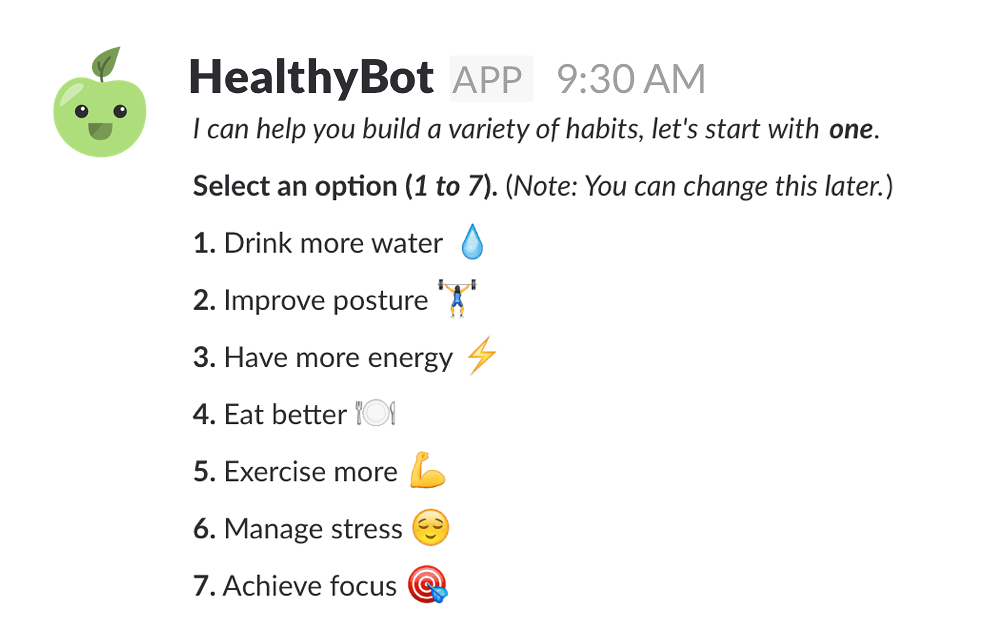
\includegraphics[width=3.5in]{../resources/existing-bots/healthy-bot.png}
  \hspace{10px}
  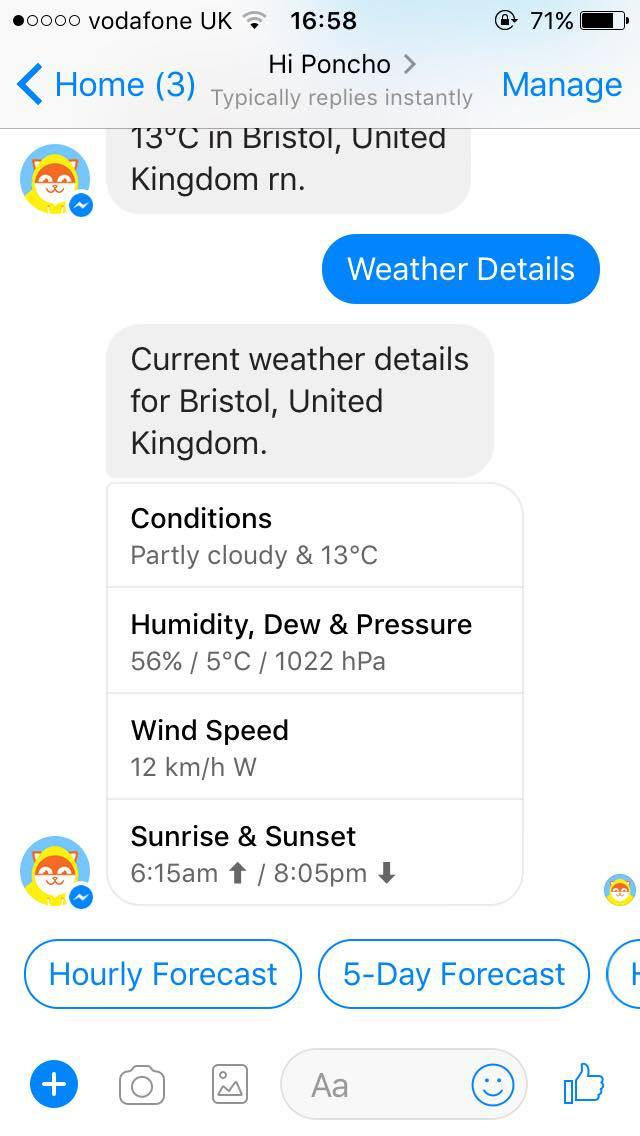
\includegraphics[width=1.9in]{../resources/existing-bots/poncho.jpg}
  \caption{Left: \textit{Healthy Bot} (\url{https://healthybot.io}): A Slack chatbot for forming new positive habits. Right: \textit{Poncho} (\url{https://poncho.is/}): An example of Facebook Messenger Weather Chatbot}
  \label{fig:healthy_bot_and_poncho}
\end{figure}


\subsection*{Facebook Messenger}

Interaction with Facebook Messenger chatbots is varied. Existing bots use three methods of interaction that utilise different Facebook Messenger UI paradigms. First, NLP is fully utilised. The bot sits patiently until it receives a message, then it sends the message off to a service that performs processing and returns the message breakdown. The bot then chooses an action based on the message. For example, the Poncho weather bot (\url{https://poncho.is/}) displays the forecast for Bristol if you message \textit{bristol forecast}. As previously discussed this method of interaction does not suit our needs because we do not require users to ask questions to the bot.



Second, NLP is not used at all and Quick Replies are heavily utilised. Everist (\url{https://www.everist.ai/}) and Cleo (\url{https://meetcleo.com/}) bots use Quick Replies almost like a menu with a set of options. After users message the bot once, the set of quick replies returns to encourage users to only use these as the method of communication. Although this makes coding the prototype easier, it is difficult to get \textit{free text} from users. Finally, Joy (\url{http://www.hellojoy.ai/}) uses a combination of free text and quick replies to set-up users and interact with them every day. This is the combination that Harry's Habits will use to get free text from users and enable quick choice from a menu of actions.

\begin{figure}[H]
  \centering
  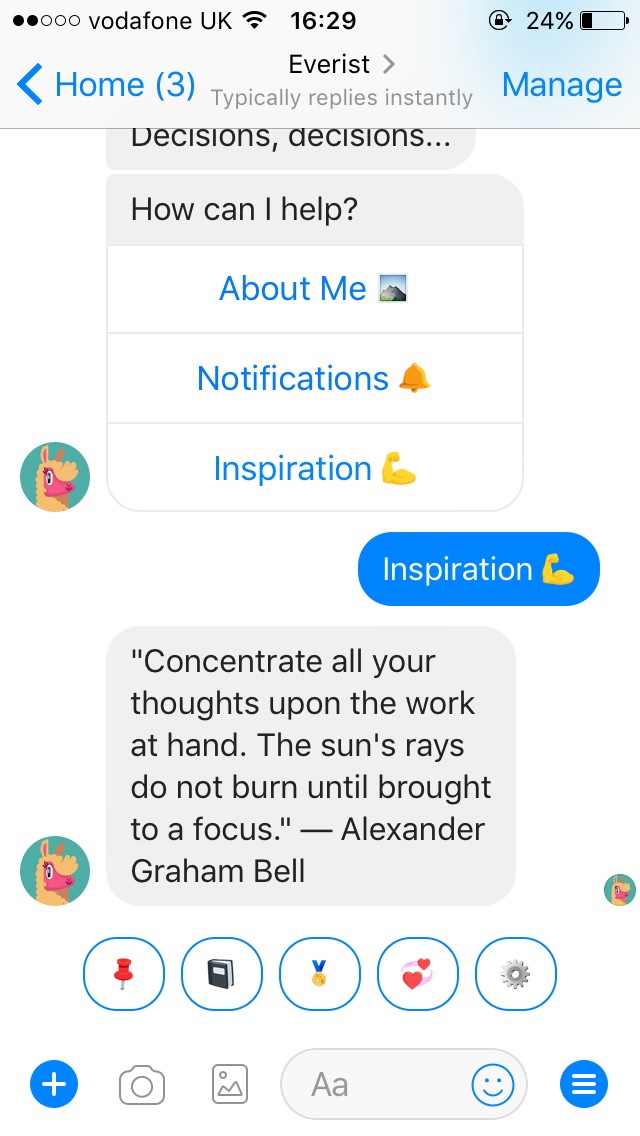
\includegraphics[width=1.9in]{../resources/existing-bots/everist.png}
  \hspace{10px}
  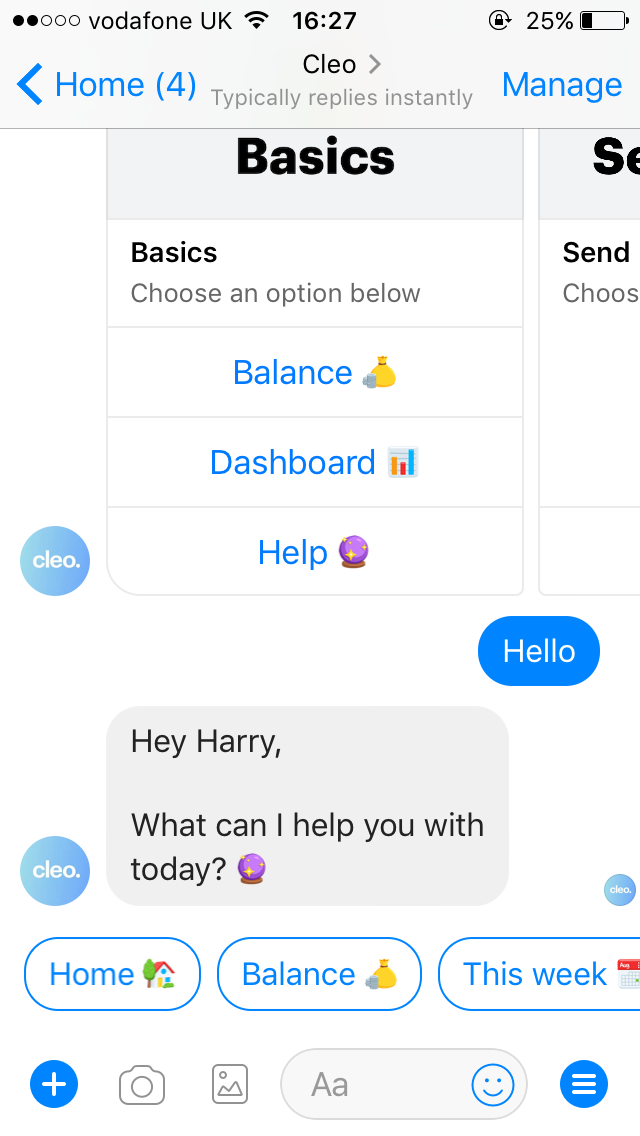
\includegraphics[width=1.9in]{../resources/existing-bots/cleo.png}
  \hspace{10px}
  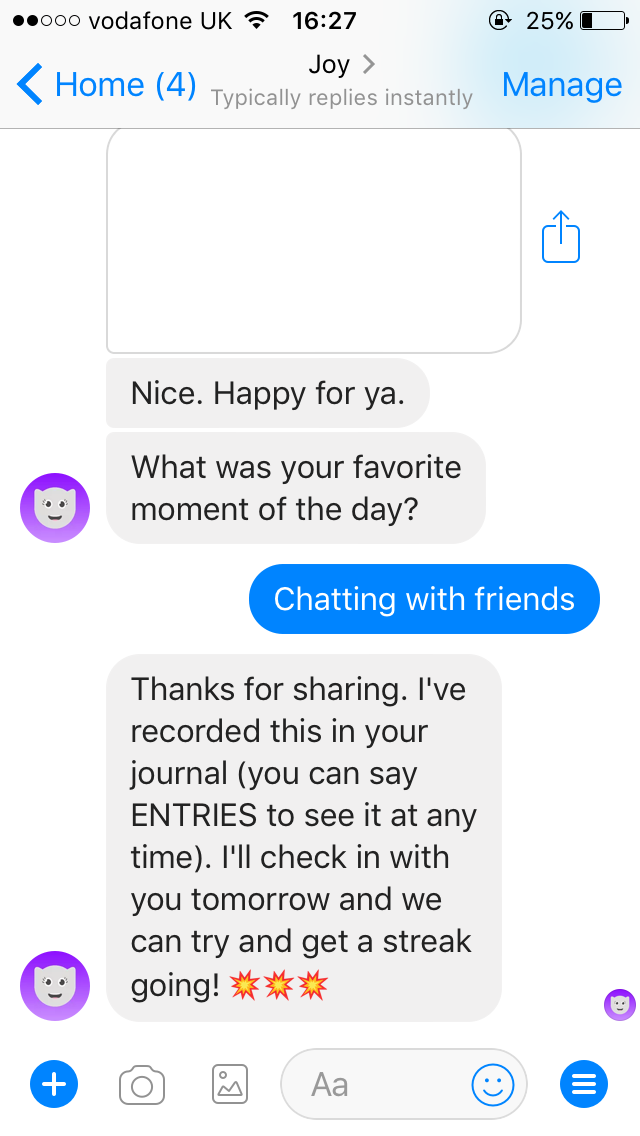
\includegraphics[width=1.9in]{../resources/existing-bots/joy-ai.png}
  \caption{Examples of chatbots performing different actions}
  \label{fig:chatbots_examples}
\end{figure}


\subsection*{Supporting Habit Formation}
Harry's Habits is built into an existing social network that people are used to and will track habits and deliver rewards. The social scaffolding around the interaction with the bot will help reinforce the response to notifications, as people are more likely to respond to the bot because they could perceive the bot as a real person as it is located in a list next to their other contacts. The bot will track simple actions of similar difficulty to reduce the amount of time needed before the action turns into a habit~\cite{article_how_habits_formed_modelling_habit_formation}. Other design methods to help people form new habits were looked at but will not be added to the prototype to limit the scope. Gamification, such as using gambling elements and engineering luck into games have been shown to encourage interaction~\cite{article_free_to_play_making_money_from_games_you_give_away}. Using monetary rewards to create a feedback loop where people keep coming back for the reward~\cite{website_how_to_design_feedback_loops}. Both of these elements can help with interaction but do not build habit automaticity, therefore leading to a drop in performance when the feedback is removed.

\subsection*{Delivering Rewards}
The types of rewards are separated into three categories, visual, auditory and visual-auditory. The content of these rewards are experimented with to test if they provide user satisfaction. The rise of social media and increasing use of humorous memes was utilised to provide the motivating content of the rewards. This works well with the prototype integration into an existing social media messaging platform. These rewards will be displayed to the user within the chatbot after they complete their habit. The modalities are mapped to identify a pattern across the modes before they are implemented and adapted for delivering rewards. The rewards were aimed at motivating participants to keep coming back every day and completing their habits. Several gifs and audio files were identified that categorised themselves as motivational and each gif file was vaguely matched and tweaked to match the audio frequency. The relationship between the audio and the visual is inferred, therefore this mapping is \textit{semi-congruent}.

\begin{figure}[H]
  \centering
  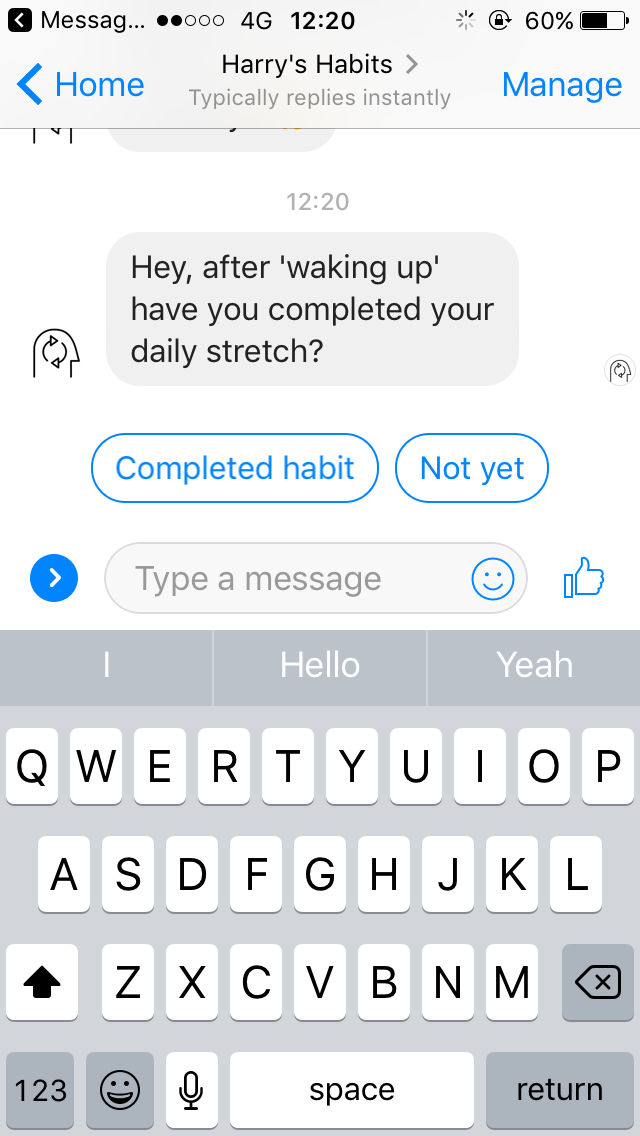
\includegraphics[width=1.5in]{resources/figures/reminder.png}
  \hspace{10px}
  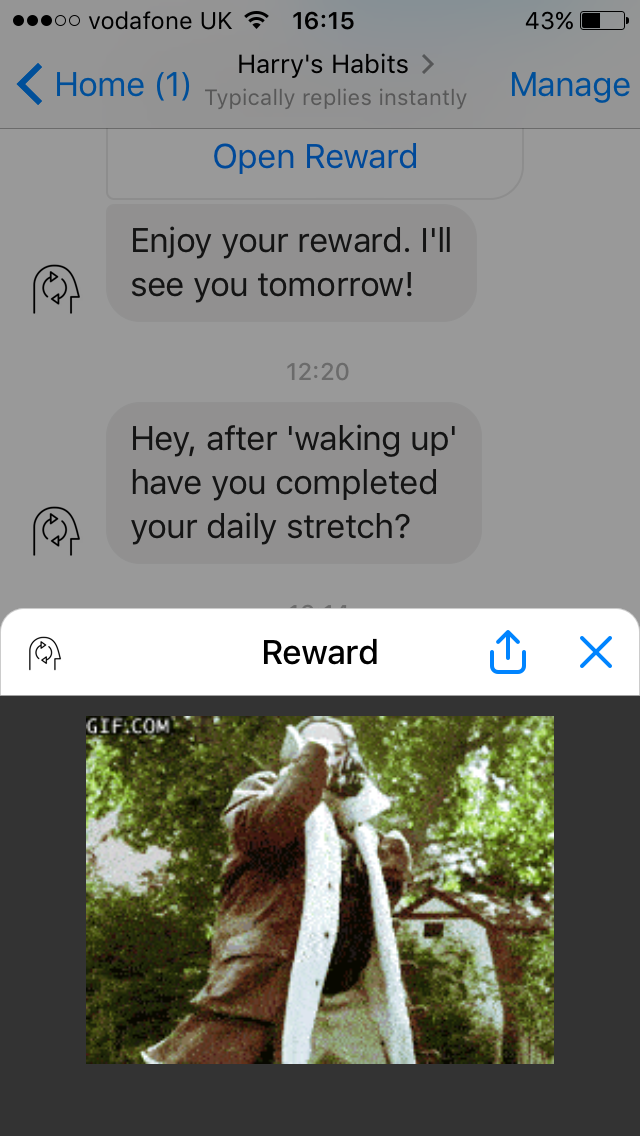
\includegraphics[width=1.5in]{resources/figures/reward-visual.png}
  \caption{Harry's Habits delivering a back-up notification and a visual reward.}
  \label{fig:setup_media_1}
\end{figure}


There are two different methods of delivering visual, auditory and visual-auditory rewards to users. First, gifs and audio sent as a message to the user (inline). This has the benefit of being native to Messenger, providing a better user experience and is faster to receive, requiring less buttons to be pressed. However, each reward was not displayed consistently. Visual rewards started as soon as they were delivered, but the auto reward had a \textit{play} button that had to be pressed before the audio started and the visual-auditory rewards also had a button that needed to be pressed. Inconsistency with delivery would make it difficult to evaluate the effectiveness of each reward. Therefore the second method is chosen to allow for consistency when delivering rewards.

\begin{figure}[H]
  \centering
  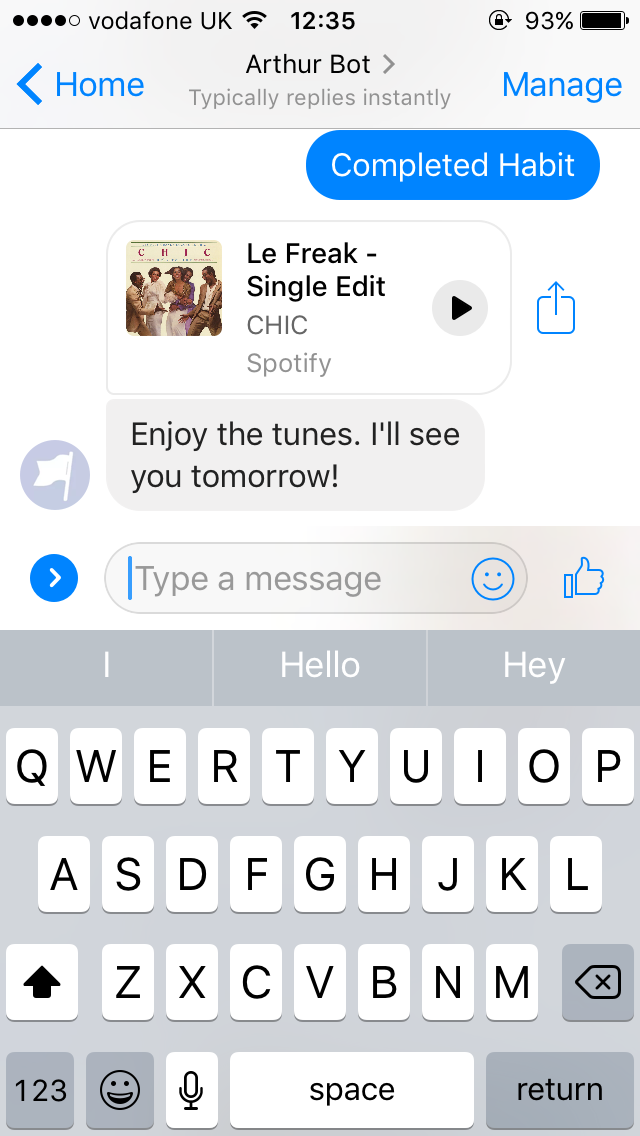
\includegraphics[width=1.5in]{../resources/design/reward-audio-inline.png}
  \hspace{10px}
  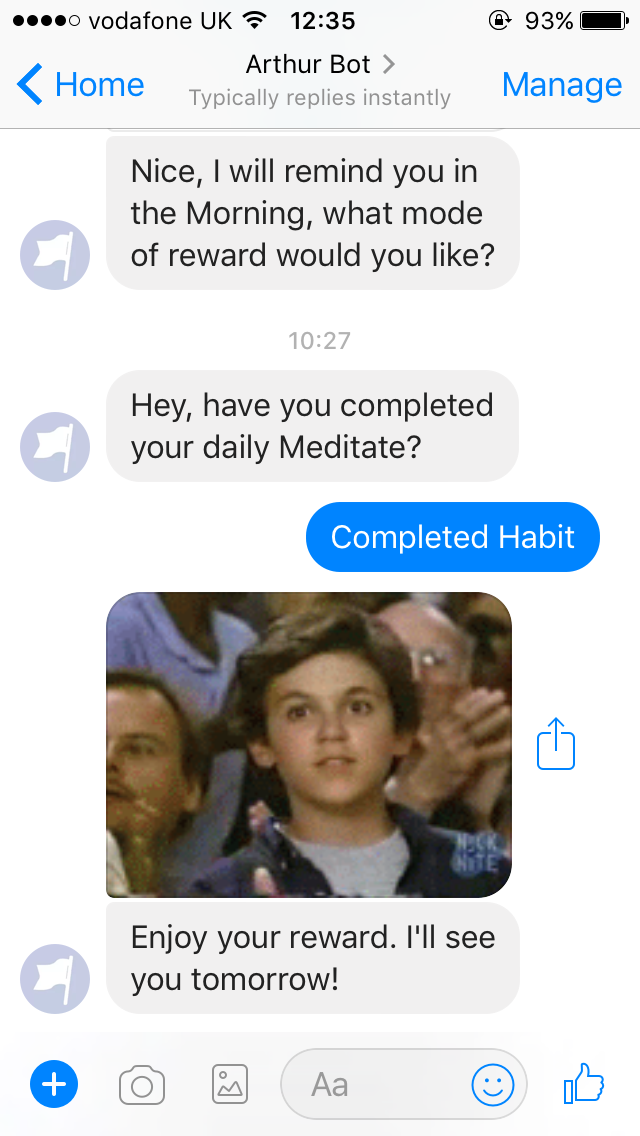
\includegraphics[width=1.5in]{../resources/design/reward-visual-inline.png}
  \caption{Auditory and visual inline rewards.}
  \label{fig:rewards_inline}
\end{figure}


\begin{figure}[H]
  \centering
  \includegraphics[width=1.5in]{../resources/design/reward-visual-2.png}
  \hspace{10px}
  \includegraphics[width=1.5in]{../resources/design/reward-audio.png}
  \caption{Consistency between every reward, even across devices. Left, visual reward, right, auditory reward.}
  \label{fig:rewards_consistency}
\end{figure}



\newpage


\subsection{User Flows} \label{user_flow}
Full user interaction from setup to completing a reward was designed. This setup used a combination of Quick Replies and free text to gather demographic information and complete the setup for each user. Harry's Habits logo was design by the Noun Project by Yu luck (\url{https://thenounproject.com/term/custom/402041/}).

\begin{itemize}
  \item \textbf{Setup}
  \begin{itemize}
    \item Press button that opens the bot in the Facebook Messenger app.
    \item Answer a series of setup questions to the bot via the Facebook Messenger app.
    \item User chooses an existing habit they would like to develop from a list.
    \item User supplies an existing routine to integrate their new habit into.
    \item User chooses a time the existing routine normally happens.
    \item User finishes the setup and closes the Facebook Messenger app.
  \end{itemize}
  \item \textbf{Trigger}
  \begin{itemize}
    \item At the time of the existing routine the user performs their chosen habit.
    \item The user receives a notification after the routine, asking if they managed to complete their habit or if they need more time.
    \item If they need more time, the notification will \textit{snooze} for about an hour and be sent again.
    \item If users regularly snooze they will be asked if the time of their existing routine has changed.
    \item If users say they have completed their habit, they will be sent a message Quick Reply that leads to a reward.
  \end{itemize}
  \item \textbf{Reward}
  \begin{itemize}
    \item Users will press the reward button that will take them to a website that contains a link to open a reward. This allows the experience to be consistent for each reward modality.
    \item User will receive a reward from one of the following modalities:
    \begin{itemize}
      \item Visual: video with no sound
      \item Audio: soundtrack
      \item Visual-Auditory: video with sound
    \end{itemize}
  \end{itemize}
\end{itemize}

\subsubsection{Setup Flow} \label{setup_flow}

\begin{figure}[H]
  \centering
  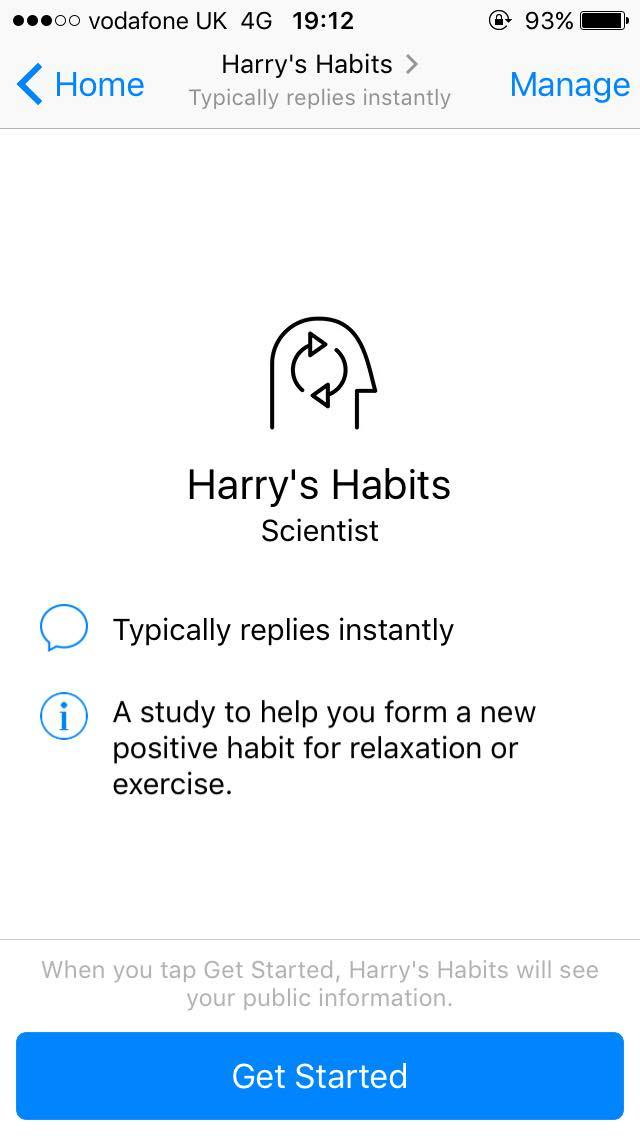
\includegraphics[width=1.4in]{resources/design/process/1.jpg}
  \hspace{10px}
  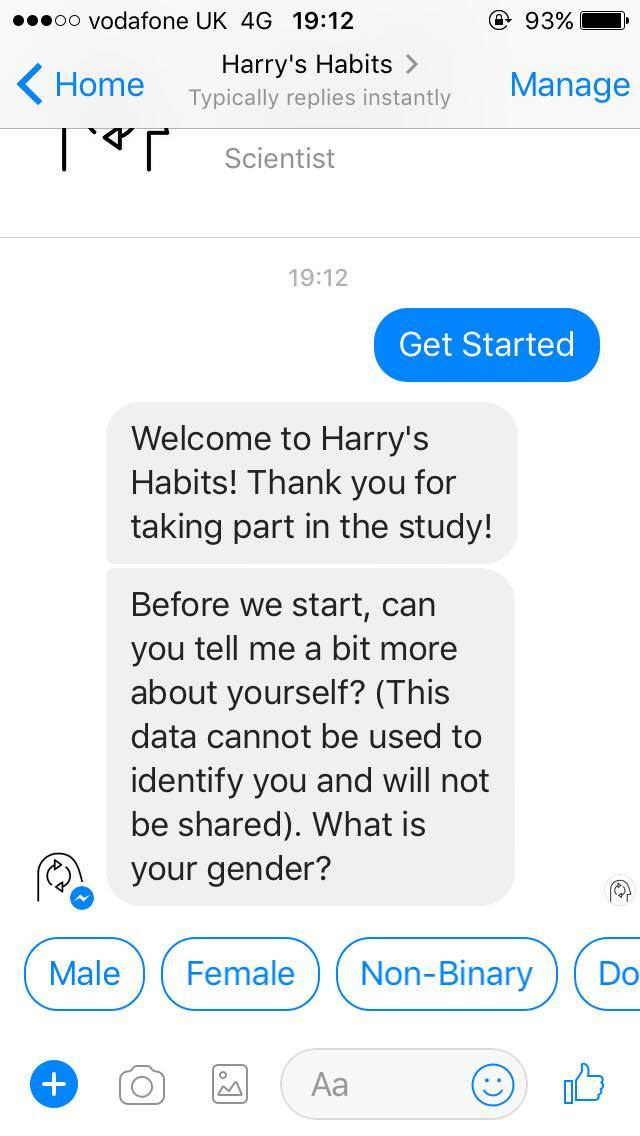
\includegraphics[width=1.4in]{resources/design/process/2.jpg}
  \hspace{10px}
  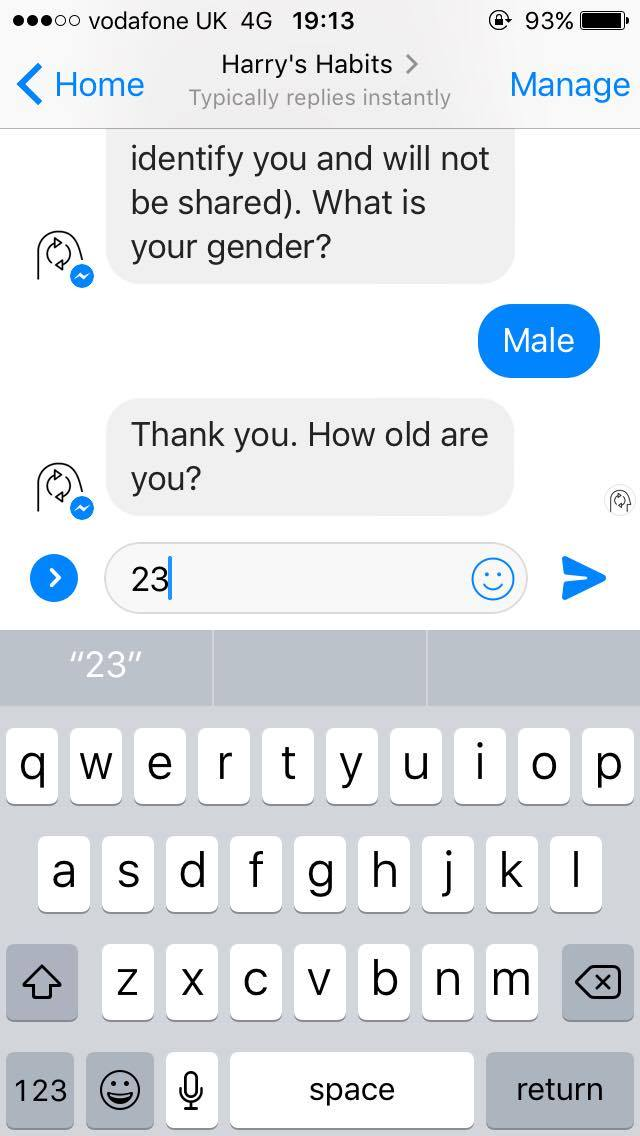
\includegraphics[width=1.4in]{resources/design/process/3.jpg}
  \hspace{10px}
  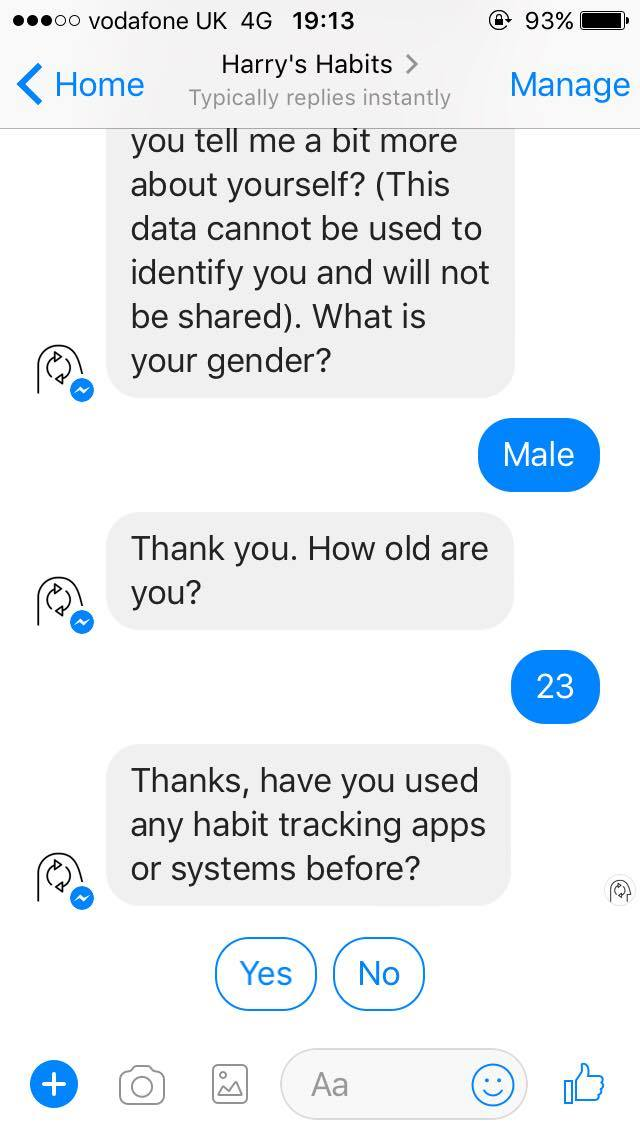
\includegraphics[width=1.4in]{resources/design/process/4.jpg}
  \newline
  \newline
  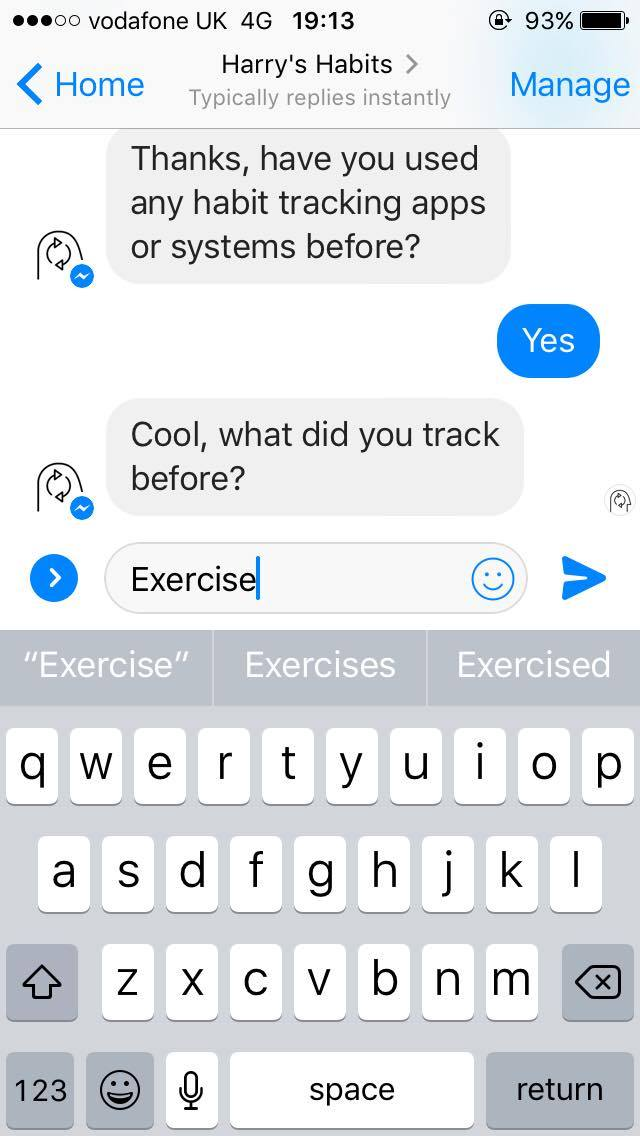
\includegraphics[width=1.4in]{resources/design/process/5.jpg}
  \hspace{10px}
  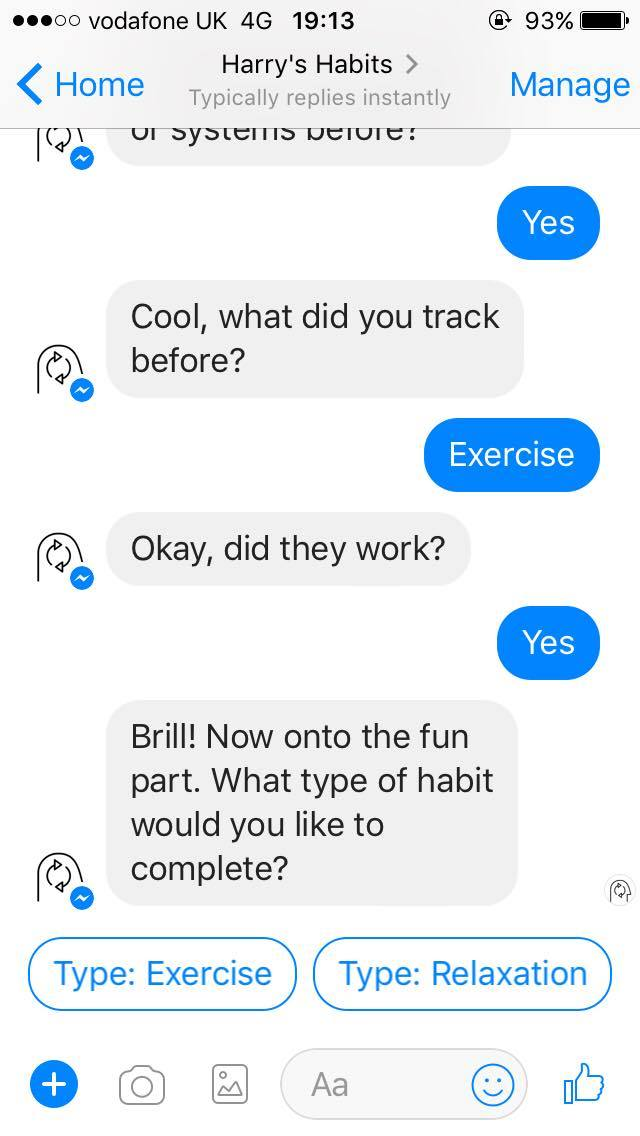
\includegraphics[width=1.4in]{resources/design/process/6.jpg}
  \hspace{10px}
  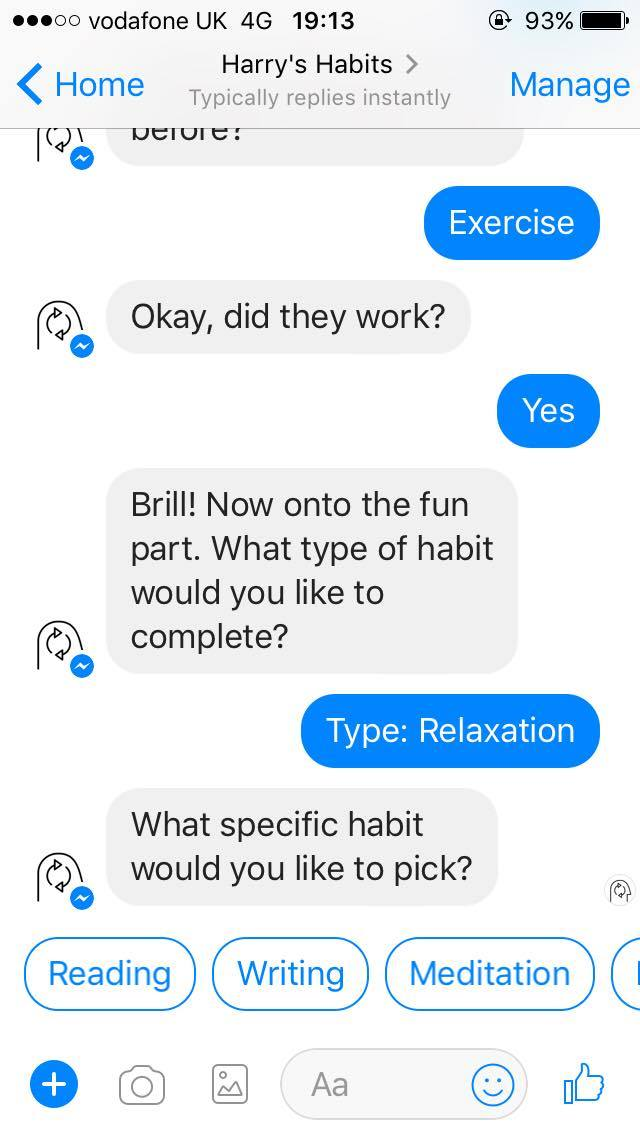
\includegraphics[width=1.4in]{resources/design/process/7.jpg}
  \hspace{10px}
  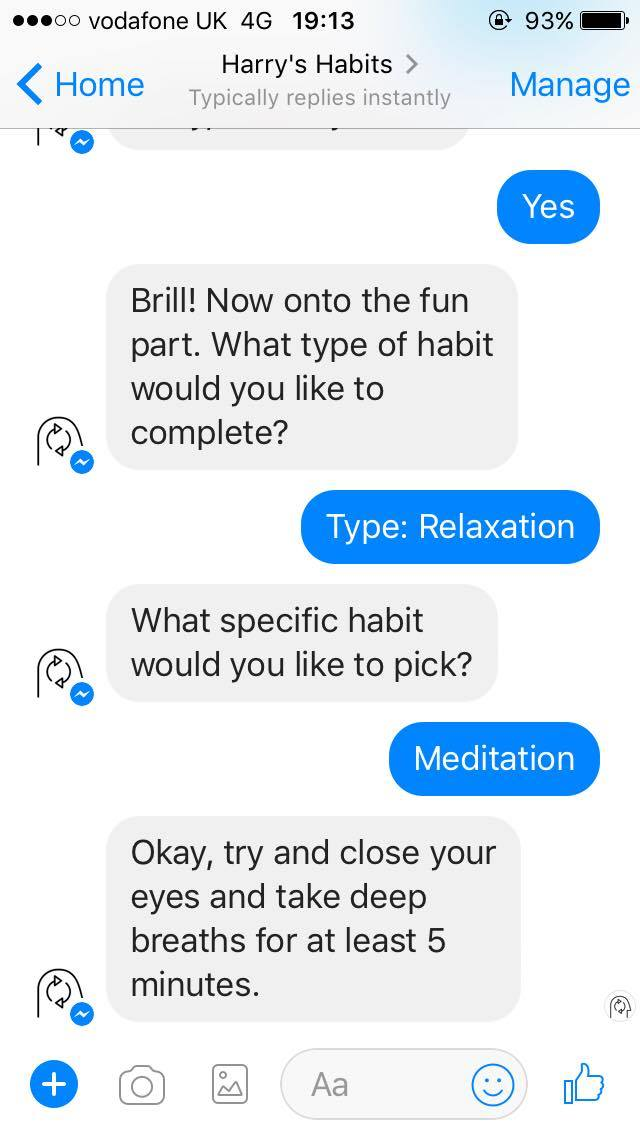
\includegraphics[width=1.4in]{resources/design/process/8.jpg}
  \newline
  \newline
  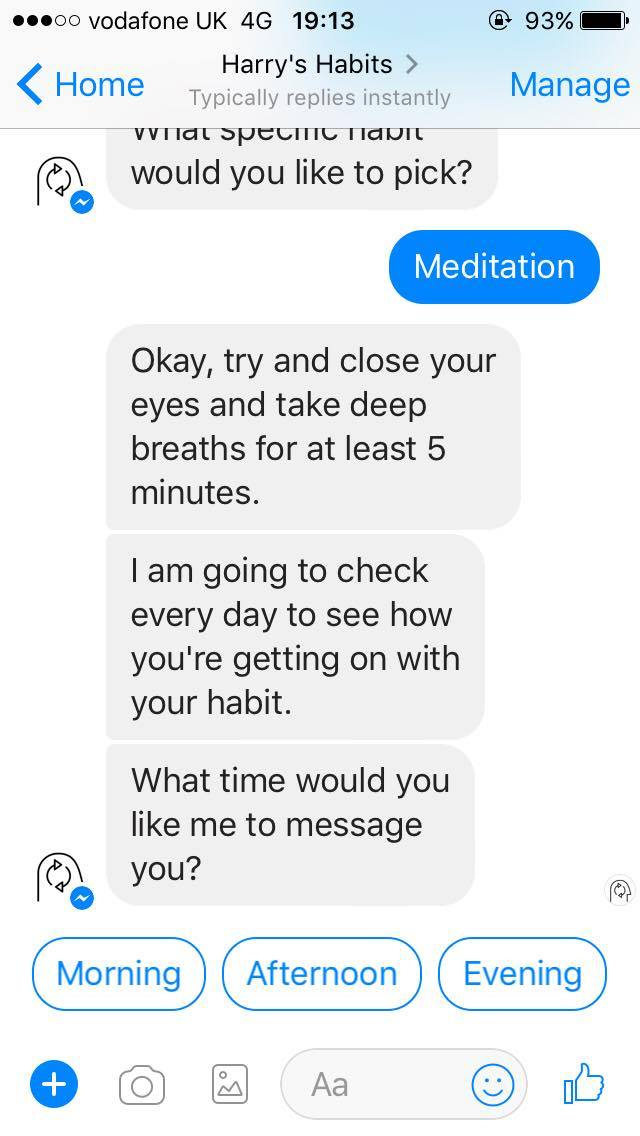
\includegraphics[width=1.4in]{resources/design/process/9.jpg}
  \hspace{10px}
  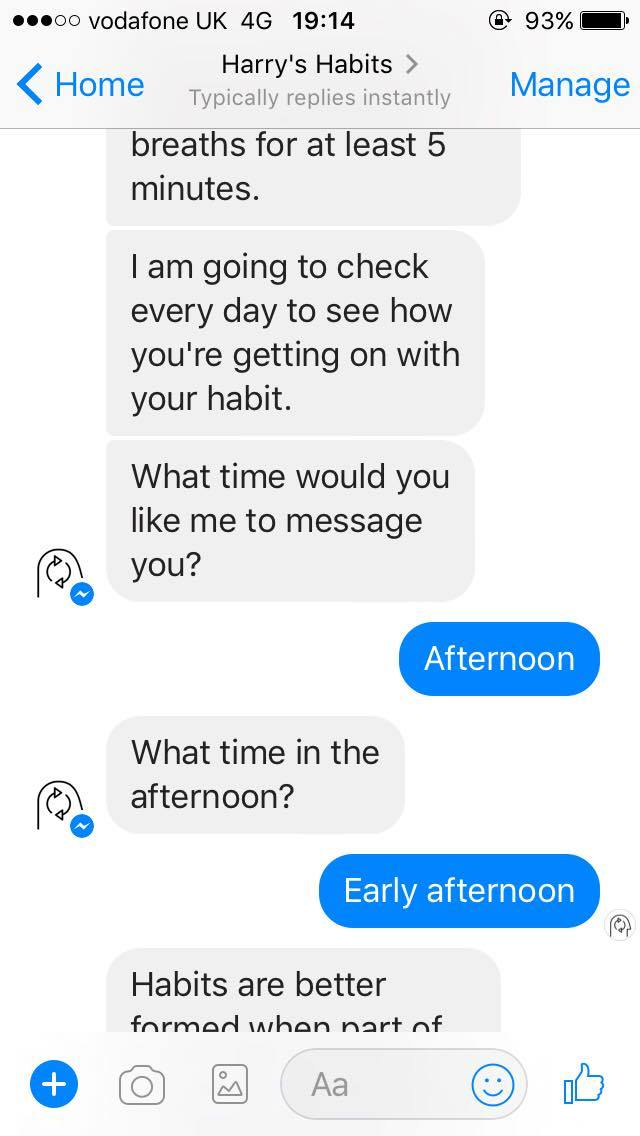
\includegraphics[width=1.4in]{resources/design/process/10.jpg}
  \hspace{10px}
  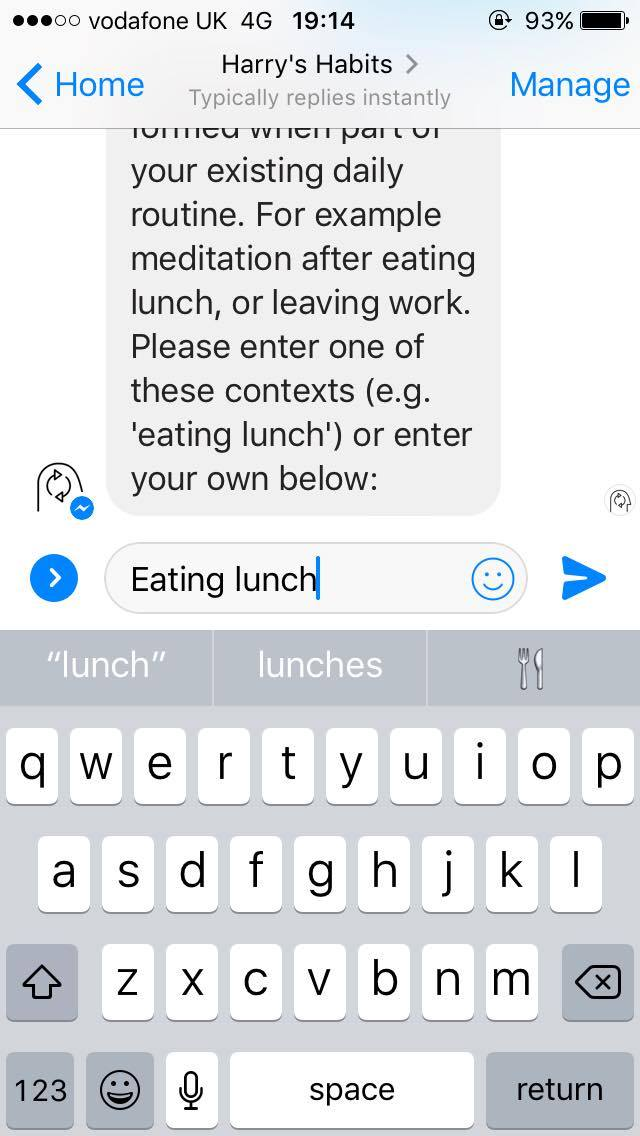
\includegraphics[width=1.4in]{resources/design/process/11.jpg}
  \hspace{10px}
  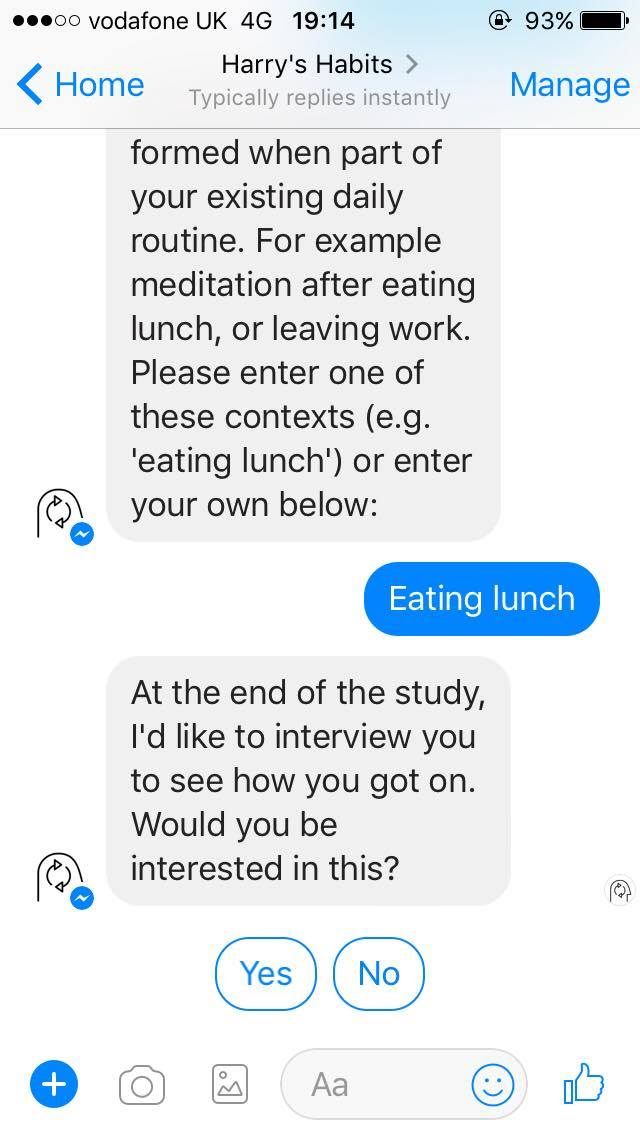
\includegraphics[width=1.4in]{resources/design/process/12.jpg}
  \caption{Setup flow for Harry's Habits.}
  \label{fig:setup_flow_screenshots}
\end{figure}

\begin{figure}[H]
  \centering
  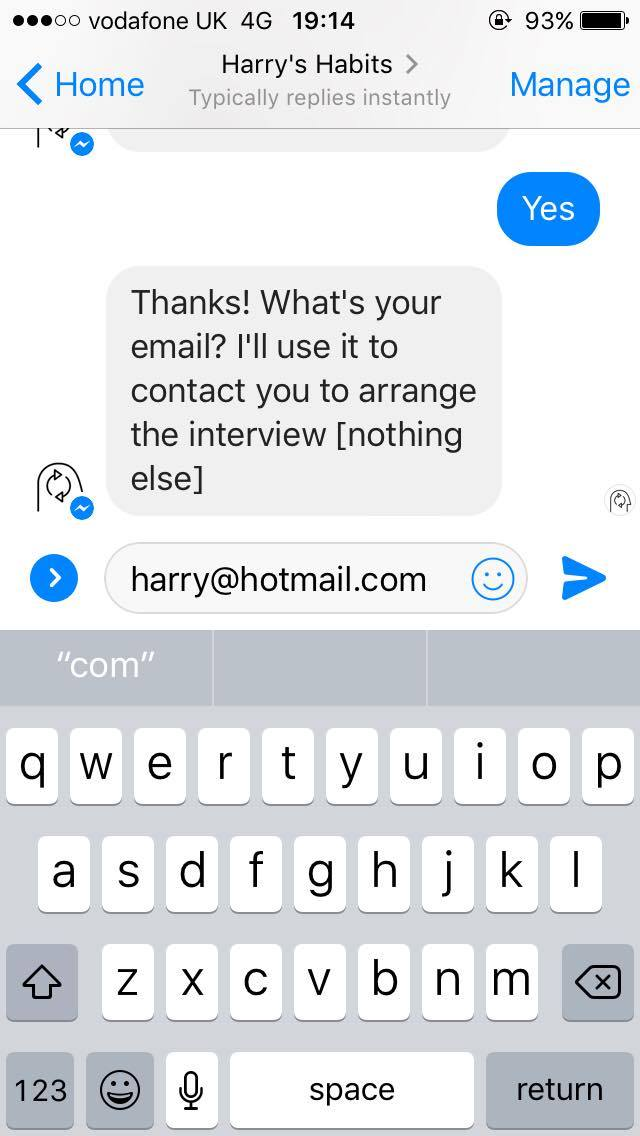
\includegraphics[width=1.5in]{resources/design/process/13.jpg}
  \hspace{10px}
  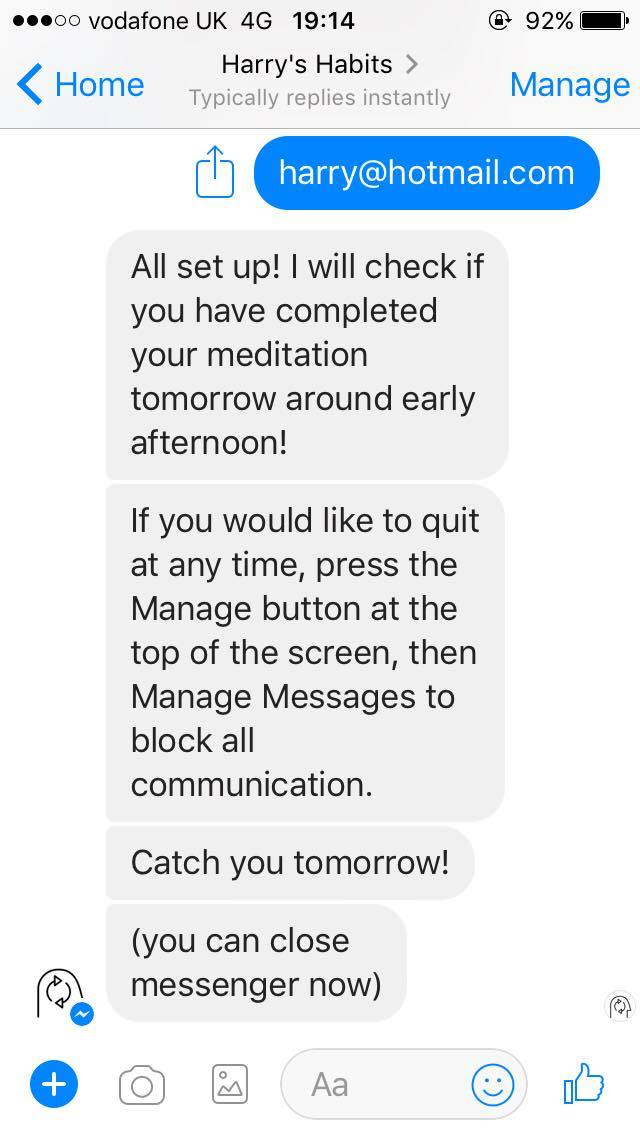
\includegraphics[width=1.5in]{resources/design/process/14.jpg}
  \hspace{10px}
  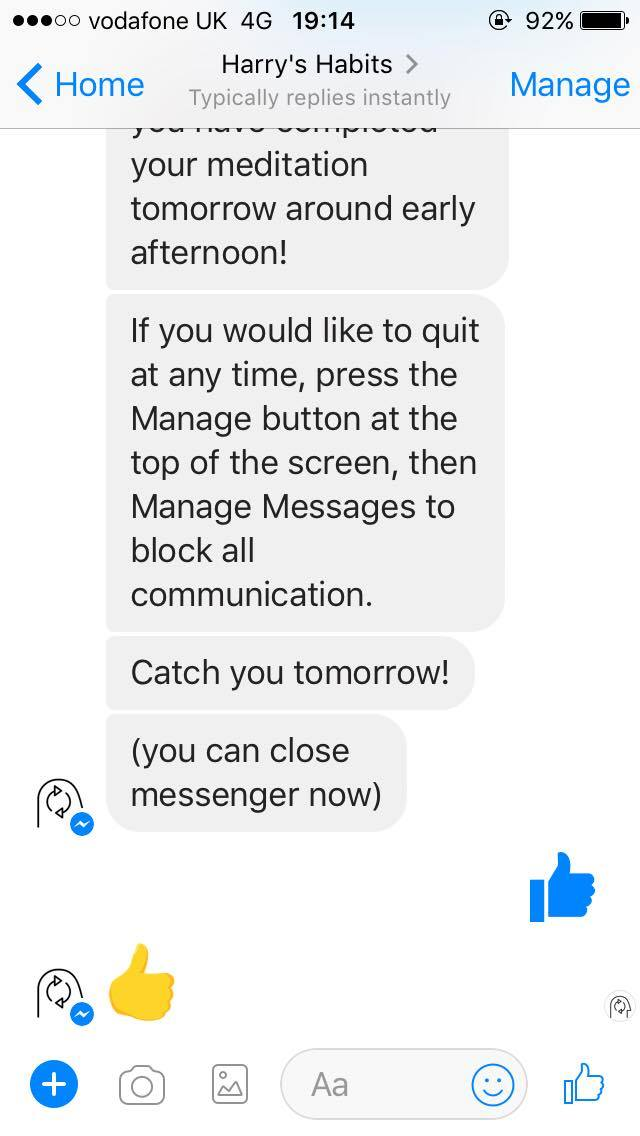
\includegraphics[width=1.5in]{resources/design/process/15.jpg}
  \caption{Continued: Setup flow for Harry's Habits.}
  \label{fig:setup_flow_screenshots_2}
\end{figure}


\subsubsection{Trigger Flow} \label{trigger_flow}

\begin{figure}[H]
  \centering
  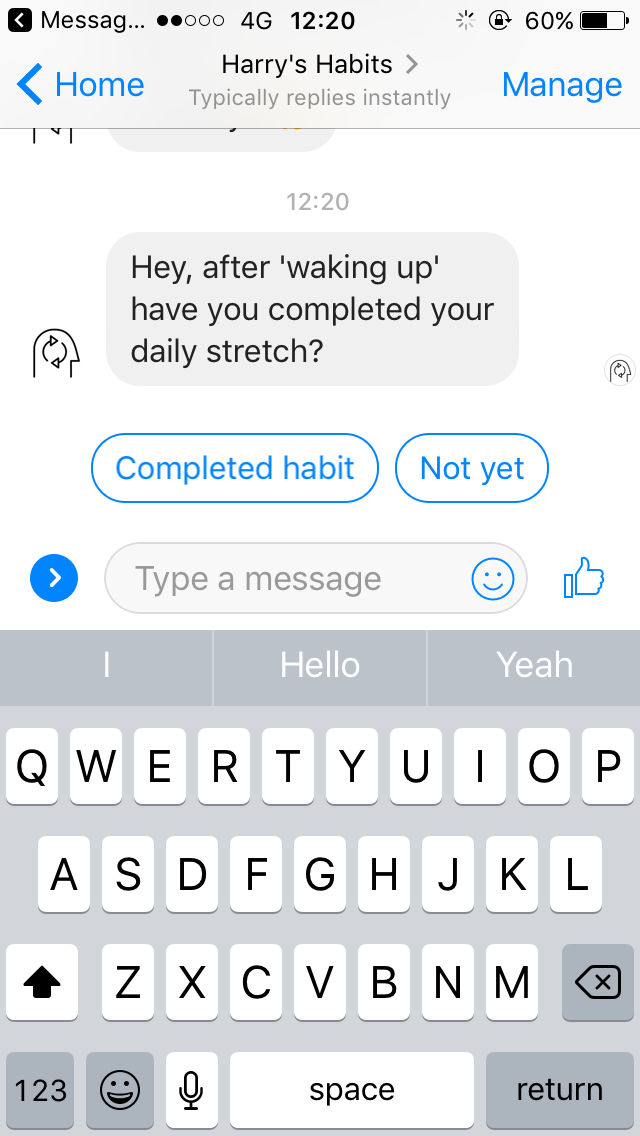
\includegraphics[width=2in]{resources/design/media/3.png}
  \hspace{10px}
  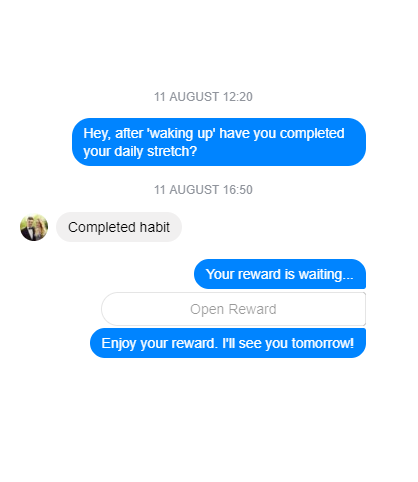
\includegraphics[width=2.8in]{resources/design/completed_habit.png}
  \caption{Trigger flow for Harry's Habits.}
  \label{fig:trigger_flow_screenshots}
\end{figure}


\subsubsection{Reward Flow} \label{reward_flow}

\begin{figure}[H]
  \centering
  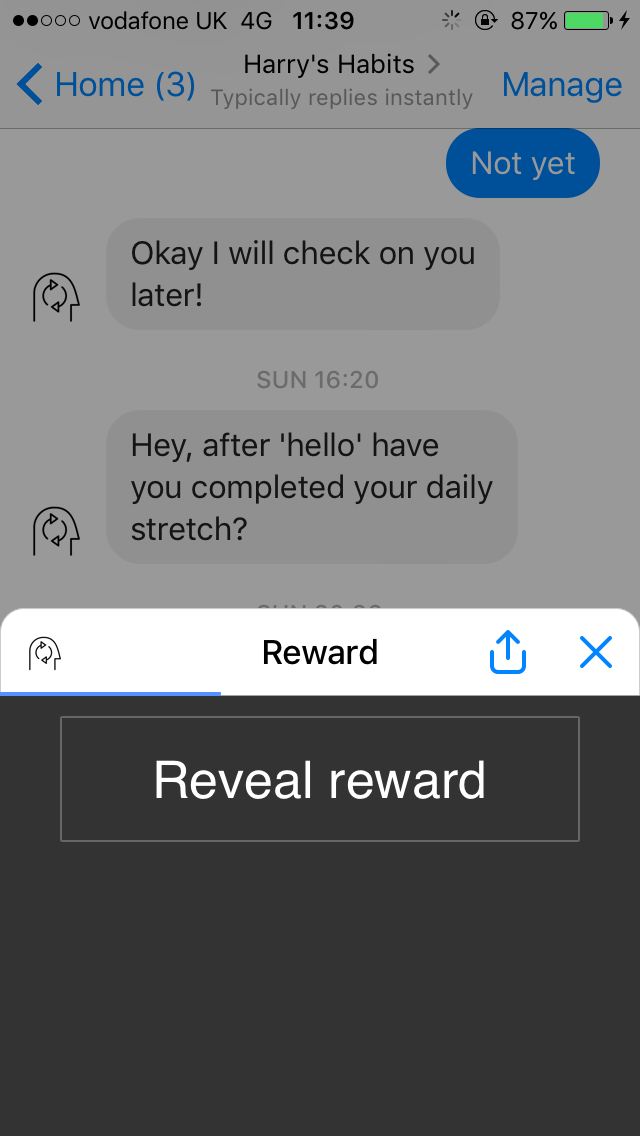
\includegraphics[width=2in]{resources/design/reward-visual-1.png}
\end{figure}
\begin{figure}[H]
  \centering
  \includegraphics[width=1.6in]{resources/design/reward-visual-2.png}
  \hspace{5px}
  \includegraphics[width=1.6in]{resources/design/reward-audio.png}
  \hspace{5px}
  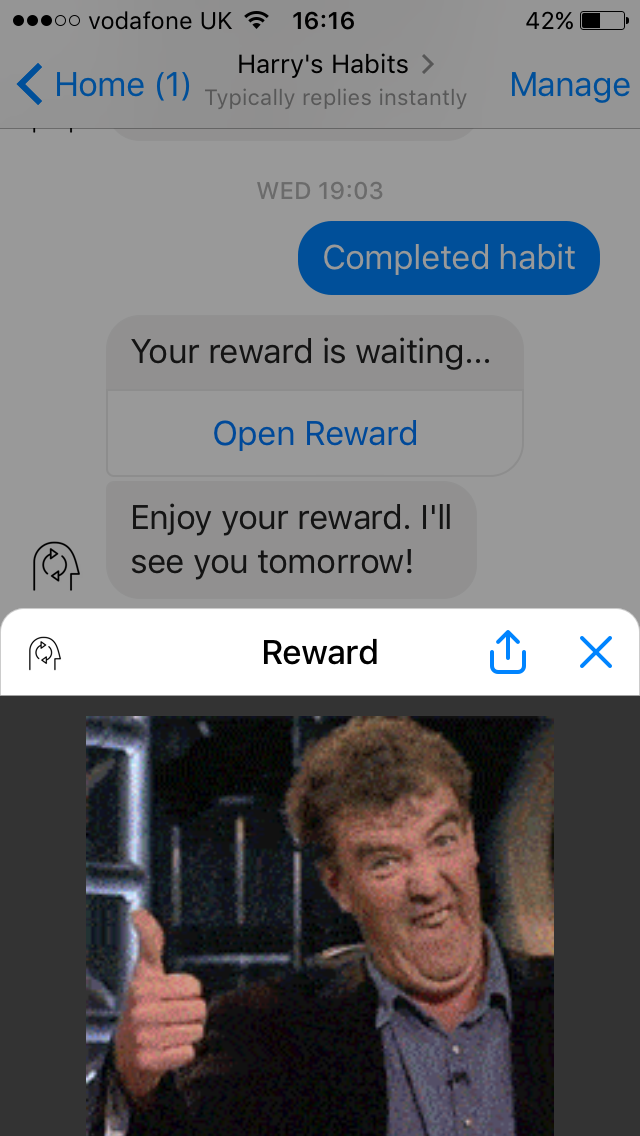
\includegraphics[width=1.6in]{resources/design/reward-visual-gif-2.png}
  \caption{Reward flow for visual, auditory and visual-auditory rewards for Harry's Habits.}
  \label{fig:reward_flow_screenshots}
\end{figure}

\newpage
